\documentclass[11pt]{article}
\usepackage[utf8]{inputenc}
\usepackage[T1]{fontenc}
\usepackage{amsmath,amssymb}
\usepackage{graphicx}
\usepackage{booktabs}
\usepackage[margin=1in]{geometry}
\usepackage{caption}
\usepackage[hidelinks]{hyperref}
\usepackage{float}

\renewcommand{\thetable}{S\arabic{table}}
\renewcommand{\thefigure}{S\arabic{figure}}

\title{\textbf{Supplementary Information}\\[6pt]
\large Sparse autoencoders reveal organized biological knowledge but minimal regulatory
logic in single-cell foundation models}
\author{Ihor Kendiukhov}
\date{}


\begin{document}

\maketitle

\section*{Supplementary Tables}

\begin{table}[htbp]
\centering
\caption{\textbf{Composition of the control cohorts.} Cells per line.}
\label{tab:cohorts}
\smallskip
\small
\begin{tabular}{lrrrrr}
\toprule
Cohort & K562 & RPE1 & Jurkat & HepG2 & Total \\
\midrule
Non-targeting cells in the resource & 10,691 & 11,485 & 12,013 & 4,976 & 39,165 \\
Atlas extraction cohort & 581 & 567 & 591 & 261 & 2,000 \\
Causal-patching cohort & 0 & 0 & 0 & 200 & 200 \\
\bottomrule
\end{tabular}
\\[2pt]
\footnotesize The control condition is defined by perturbation label, so the cohort spans every cell line in the resource. The cohort reported here was reproduced from the extraction procedure under its recorded seed and validated against the per-cell gene counts stored at extraction time: all 25 cells checked match.
\end{table}

\begin{table}[H]
\centering
\caption{\textbf{Per-ontology enrichment counts across all 18 Geneformer layers.} Each entry is the number of significant enrichments (FDR $< 0.05$) for features at that layer. GO~BP = Gene Ontology Biological Process. TRRUST columns show enrichment for TF target sets (TF) and individual TF$\to$target edges (Edges).}
\label{tab:perontology}
\smallskip
\begin{tabular}{rrrrrrc}
\toprule
Layer & GO BP & KEGG & Reactome & STRING & TRRUST TF & TRRUST Edges \\
\midrule
0  & 10,153 & 2,650 & 11,001 & 302 & 155 & 42 \\
1  & 10,022 & 2,433 & 10,512 & 258 & 164 & 48 \\
2  & 9,948  & 2,495 & 10,790 & 283 & 150 & 32 \\
3  & 9,726  & 2,514 & 9,525  & 273 & 157 & 37 \\
4  & 8,537  & 2,045 & 9,195  & 248 & 133 & 30 \\
5  & 7,695  & 1,845 & 8,189  & 216 & 136 & 24 \\
6  & 7,180  & 1,555 & 7,871  & 182 & 110 & 28 \\
7  & 6,628  & 1,637 & 7,080  & 181 & 125 & 30 \\
8  & 6,850  & 1,570 & 7,169  & 199 & 90  & 27 \\
9  & 7,299  & 1,643 & 7,880  & 207 & 103 & 29 \\
10 & 8,461  & 1,751 & 9,247  & 214 & 128 & 30 \\
11 & 8,785  & 2,089 & 8,957  & 227 & 112 & 31 \\
12 & 8,217  & 1,915 & 8,856  & 210 & 117 & 35 \\
13 & 7,158  & 1,686 & 8,393  & 202 & 101 & 28 \\
14 & 7,615  & 1,595 & 8,412  & 221 & 97  & 27 \\
15 & 6,790  & 1,520 & 7,135  & 150 & 126 & 34 \\
16 & 7,040  & 1,781 & 7,172  & 158 & 87  & 25 \\
17 & 7,002  & 1,762 & 6,869  & 193 & 131 & 25 \\
\midrule
\textbf{Total} & \textbf{145,106} & \textbf{34,486} & \textbf{154,253} & \textbf{3,924} & \textbf{2,222} & \textbf{562} \\
\bottomrule
\end{tabular}
\end{table}

\begin{table}[H]
\centering
\caption{\textbf{Cross-layer feature persistence from layer~0.} Matches = features at L0 with cosine similarity $> 0.7$ to any feature at the target layer. The model undergoes radical representational transformation: by layer~6, essentially all features are novel with no L0 ancestry.}
\label{tab:persistence}
\smallskip
\begin{tabular}{lcc}
\toprule
L0 $\to$ Target & Matches (cos $> 0.7$) & Rate \\
\midrule
L0 $\to$ L1  & 114 & 2.5\% \\
L0 $\to$ L2  & 93 & 2.0\% \\
L0 $\to$ L4  & 67 & 1.5\% \\
L0 $\to$ L6  & 25 & 0.5\% \\
L0 $\to$ L8  & 10 & 0.2\% \\
L0 $\to$ L10 & 1 & $\sim$0\% \\
L0 $\to$ L12+ & 0 & 0\% \\
\bottomrule
\end{tabular}
\end{table}

\begin{table}[H]
\centering
\caption{\textbf{Co-activation module statistics across all 18 layers.} PMI-based graphs with Leiden clustering (resolution = 1.0). Modules = number of distinct communities. Coverage = fraction of alive features in at least one module.}
\label{tab:modules_full}
\smallskip
\begin{tabular}{rccrc}
\toprule
Layer & Modules & Feats in Modules & PMI Edges & Coverage \\
\midrule
0  & 6  & 4,577 & 446,324 & 99.3\% \\
1  & 8  & 4,562 & 440,681 & 99.0\% \\
2  & 7  & 4,536 & 404,403 & 98.6\% \\
3  & 8  & 4,518 & 393,574 & 98.3\% \\
4  & 9  & 4,502 & 393,194 & 98.2\% \\
5  & 12 & 4,472 & 390,845 & 97.7\% \\
6  & 7  & 4,458 & 383,033 & 97.3\% \\
7  & 8  & 4,439 & 371,832 & 96.7\% \\
8  & 7  & 4,478 & 369,280 & 97.6\% \\
9  & 7  & 4,535 & 380,304 & 98.7\% \\
10 & 9  & 4,571 & 388,498 & 99.3\% \\
11 & 8  & 4,565 & 388,103 & 99.3\% \\
12 & 7  & 4,567 & 388,977 & 99.5\% \\
13 & 7  & 4,561 & 383,779 & 99.5\% \\
14 & 8  & 4,543 & 379,595 & 99.5\% \\
15 & 8  & 4,461 & 340,269 & 98.2\% \\
16 & 8  & 4,358 & 327,895 & 96.0\% \\
17 & 7  & 4,474 & 343,059 & 97.7\% \\
\midrule
\textbf{Total} & \textbf{141} & & & \\
\bottomrule
\end{tabular}
\end{table}

\begin{table}[H]
\centering
\caption{\textbf{Geneformer cross-layer information highways.} PMI between SAE feature activations at source and target layers (500K positions each). A highway = source feature with $\geq$1 target-layer feature at PMI $> 3$. \textbf{Note:} the numbers here use the main-atlas 500K-position protocol; Table~\ref{tab:highways_null} reports the same three pairs recomputed on a 100K-position subsample with a permutation-null control. The two sets of numbers differ by less than one percentage point (e.g.\ L0$\to$L5: 98.4\% here vs.\ 98.96\% in Table~\ref{tab:highways_null}) because of the different subsample sizes, and the null correction does not change the 100K numbers.}
\label{tab:highways}
\smallskip
\begin{tabular}{lccccc}
\toprule
Layer Pair & Feats w/ Deps & Mean Max PMI & Median Max PMI & Max PMI & Highways \\
\midrule
L0 $\to$ L5   & 4,604 & 6.61 & 6.72 & 11.10 & 4,530 (98.4\%) \\
L5 $\to$ L11  & 4,518 & 6.63 & 6.71 & 10.87 & 4,401 (97.4\%) \\
L11 $\to$ L17 & 4,555 & 6.79 & 6.86 & 10.66 & 4,544 (99.8\%) \\
\bottomrule
\end{tabular}
\end{table}

\begin{table}[H]
\centering
\caption{\textbf{Null-corrected cross-layer highway fractions for the three long-range Geneformer pairs.} 100K gene positions subsampled from the K562 activation cache, encoded through the per-layer SAEs, cross-layer PMI computed as in Methods. Columns: observed 99th percentile of cross-layer PMI, permutation-null 99th percentile ($\tau_{\text{null}}^{p99}$, max across 20 column-shuffle rounds), effective threshold $\tau = \max(3.0, \tau_{\text{null}}^{p99})$, and highway fraction. The permutation null's 99th-percentile PMI is \emph{below} 3.0 in every pair tested, so the fixed threshold $\tau{=}3.0$ is already conservative and the null correction leaves the highway fraction unchanged. This argues that the $\sim$97--99\% highway rate is not an artifact of the $k{=}32$ TopK sparsity.}
\label{tab:highways_null}
\smallskip
\small
\begin{tabular}{rrrrrrr}
\toprule
Src & Tgt & Obs $p99$ PMI & Null $p99$ PMI & $\tau_\text{eff}$ & Fixed-$\tau$ highway\% & Null-corr highway\% \\
\midrule
L0  & L5  & 4.76 & 2.46 & 3.00 & 98.96\% & 98.96\% \\
L5  & L11 & 4.93 & 2.76 & 3.00 & 96.66\% & 96.66\% \\
L11 & L17 & 4.77 & 2.85 & 3.00 & 99.02\% & 99.02\% \\
\bottomrule
\end{tabular}
\end{table}

\begin{table}[H]
\centering
\caption{\textbf{Consecutive-layer highway fractions L$_i$$\to$L$_{i+1}$ (Geneformer, fixed-$\tau$).} Same protocol as Table~\ref{tab:highways_null} (100K gene positions per layer, fixed $\tau{=}3.0$). Because the permutation null's 99th percentile PMI is below 3.0 for every long-range pair tested in Table~\ref{tab:highways_null}, we do not re-run the permutation null on every consecutive pair. The curve is near-flat in the 94.7--99.1\% range with no sharp drop at any single transition, supporting continuous cross-layer information flow rather than concentrated bottlenecks. The slight dip at the final layer pair (L16$\to$L17) is consistent with the terminal-layer specialization reported in the section on layer-wise annotation in the main text.}
\label{tab:highways_consecutive}
\smallskip
\small
\begin{tabular}{rr}
\toprule
L$_i$$\to$L$_{i+1}$ & Highway\% \\
\midrule
L0  $\to$ L1  & 98.68\% \\
L1  $\to$ L2  & 98.74\% \\
L2  $\to$ L3  & 98.48\% \\
L3  $\to$ L4  & 98.35\% \\
L4  $\to$ L5  & 97.70\% \\
L5  $\to$ L6  & 97.09\% \\
L6  $\to$ L7  & 97.55\% \\
L7  $\to$ L8  & 96.96\% \\
L8  $\to$ L9  & 97.37\% \\
L9  $\to$ L10 & 98.24\% \\
L10 $\to$ L11 & 99.13\% \\
L11 $\to$ L12 & 99.05\% \\
L12 $\to$ L13 & 99.05\% \\
L13 $\to$ L14 & 98.87\% \\
L14 $\to$ L15 & 98.48\% \\
L15 $\to$ L16 & 96.72\% \\
L16 $\to$ L17 & 94.70\% \\
\bottomrule
\end{tabular}
\end{table}

\begin{table}[H]
\centering
\caption{\textbf{scGPT cross-layer information highways.} Same methodology as Table~\ref{tab:highways}. Note the progressive drop in downstream connectivity.}
\label{tab:scgpt_highways}
\smallskip
\begin{tabular}{lrccc}
\toprule
Layer Pair & PMI Edges & Upstream & Downstream & Max PMI \\
\midrule
L0 $\to$ L4  & 75,305 & 1,935/2,027 (95.5\%) & 1,960/2,048 (95.7\%) & 9.15 \\
L4 $\to$ L8  & 61,263 & 1,955/2,048 (95.5\%) & 1,723/2,048 (84.1\%) & 9.26 \\
L8 $\to$ L11 & 45,258 & 1,773/2,048 (86.6\%) & 1,289/2,048 (62.9\%) & 10.78 \\
\bottomrule
\end{tabular}
\end{table}

\begin{table}[H]
\centering
\caption{\textbf{Top cross-layer biological cascades.} Strongest annotated PMI connections between layer pairs. ``Unlabeled'' = the target feature lacks direct ontology annotation.}
\label{tab:cascades}
\smallskip
\small
\begin{tabular}{lp{2.6cm}p{2.6cm}p{3.2cm}r}
\toprule
Pair & Source Feature & Target Feature & Biological Logic & PMI \\
\midrule
L0$\to$L5  & Protein Processing in ER & \textit{unlabeled} & ER stress cascade & 11.10 \\
L0$\to$L5  & mTORC1 Regulation & Autophagy & mTORC1$\to$autophagy & 9.55 \\
L0$\to$L5  & Wnt Signaling & \textit{unlabeled} & Wnt pathway processing & 9.48 \\
\midrule
L5$\to$L11 & Protein Polyubiq. & \textit{unlabeled} & Protein quality control & 10.87 \\
L5$\to$L11 & Translation & \textit{unlabeled} & Translational regulation & 10.35 \\
L5$\to$L11 & RNA Splicing (neg.\ reg.) & \textit{unlabeled} & Post-transcriptional & 10.21 \\
\midrule
L11$\to$L17 & Protein Modification & Angiogenesis (pos.\ reg.) & PTM$\to$phenotype & 10.62 \\
L11$\to$L17 & COPII Vesicle Budding & Thermogenesis & Secretory$\to$metabolic & 10.29 \\
L11$\to$L17 & Actomyosin Org. & Cell Locomotion (neg.\ reg.) & Structure$\to$motility & 10.14 \\
\bottomrule
\end{tabular}
\end{table}

\begin{table}[H]
\centering
\caption{\textbf{PMI co-activation graph dimensions and peak memory (Geneformer layers 0 and 11).} Recomputed on a deterministic 500{,}000-position subsample (seed 42) of the 4{,}056{,}351 K562 token positions at each layer, with $\texttt{MIN\_COACTIVATION}{=}20$ and $\texttt{PMI\_THRESHOLD}{=}2.0$ to match the main-text co-activation pipeline (main-text numbers use the full 4M positions with $\texttt{MIN\_COACTIVATION}{=}50$). $N_\text{feat}$ = alive features at the layer. Peak RSS measured with \texttt{psutil.Process().memory\_info().rss}. The dense ($N{\times}N$) coactivation matrix accounts for $\approx$85~MB of the budget; the remaining $\sim$700~MB is the subsampled TopK index buffer and PyTorch/Python overhead.}
\label{tab:pmi_memory}
\smallskip
\small
\begin{tabular}{rrrrrrrr}
\toprule
Layer & $N_\text{feat}$ & Subsampled positions & $|E|$ (after thresh.) & Coact matrix (MB) & Peak RSS (MB) & Encode (s) & PMI (s) \\
\midrule
0  & 4{,}608 & 500{,}000 & 435{,}252 & 85 & 811 & 100.1 & 11.0 \\
11 & 4{,}608 & 500{,}000 & 356{,}894 & 85 & 864 &  93.6 & 10.3 \\
\bottomrule
\end{tabular}
\end{table}

\begin{table}[H]
\centering
\caption{\textbf{Leiden resolution sweep at Geneformer layers 0 and 11.} Module count ($\geq$3 features), mean module size, coverage (fraction of graph nodes in $\geq$3-feature modules), and Adjusted Rand Index vs.\ the baseline $\gamma{=}1.0$ partition for $\gamma \in \{0.5, 0.75, 1.0, 1.5, 2.0\}$. \textbf{Note on comparison with Table~\ref{tab:modules_full}:} this sweep is run on a deterministic 500K-position subsample with $\texttt{MIN\_COACTIVATION}{=}20$ (see caption of Table~\ref{tab:pmi_memory}), whereas the main-text module counts in Table~\ref{tab:modules_full} use the full 4{,}056{,}351 positions with $\texttt{MIN\_COACTIVATION}{=}50$. The different PMI significance thresholds produce slightly different partition sizes; at $\gamma{=}1.0$ the sweep gives 8 modules at L0 and 9 at L11, versus 6 and 8 in Table~\ref{tab:modules_full}. This disagreement is expected given the parameter change and should not be read as instability. The partition is \emph{not} stable in a strong ARI sense (ARI between $\gamma{=}1.0$ and its immediate neighbors is in the 0.17--0.26 range); instead, the co-activation graph exhibits a nested hierarchy in which low $\gamma$ collapses the graph into $\sim$2 very large communities and high $\gamma$ fragments each main community into finer subcommunities. The qualitative biological identities of modules (cell cycle, translation, metabolism, etc.) are preserved across the range; our main-text module counts correspond to the resolution-1.0 cut of this hierarchy.}
\label{tab:leiden_sweep}
\smallskip
\small
\begin{tabular}{rrrrrr}
\toprule
Layer & $\gamma$ & Modules ($\geq$3) & Mean size & Coverage & ARI vs $\gamma{=}1.0$ \\
\midrule
0  & 0.50 &  2 & 2{,}287.5 & 100.0\% & +0.027 \\
0  & 0.75 &  3 & 1{,}525.0 & 100.0\% & +0.259 \\
0  & 1.00 &  8 &    571.9 & 100.0\% & +1.000 \\
0  & 1.50 & 25 &    183.0 & 100.0\% & +0.252 \\
0  & 2.00 & 48 &     95.3 & 100.0\% & +0.117 \\
\midrule
11 & 0.50 &  2 & 2{,}282.0 & 100.0\% & +0.013 \\
11 & 0.75 &  3 & 1{,}521.3 & 100.0\% & +0.180 \\
11 & 1.00 &  9 &    507.1 & 100.0\% & +1.000 \\
11 & 1.50 & 31 &    147.2 & 100.0\% & +0.171 \\
11 & 2.00 & 56 &     81.5 & 100.0\% & +0.085 \\
\bottomrule
\end{tabular}
\end{table}

\begin{table}[H]
\centering
\caption{\textbf{SAE hyperparameter ablation at Geneformer layer~11.} Grid over expansion ratio $\in \{2\times, 4\times, 8\times\}$ and TopK sparsity $k \in \{16, 32, 64\}$, trained on the same 1M-position K562 subsample used in the main atlas (Methods), evaluated on 100K held-out positions. Columns: expansion, $k$, total features, variance explained on held-out positions, number of dead features (no activation on the 100K hold-out), mean absolute decoder--decoder cosine similarity on a 5{,}000-pair sample (a proxy for quasi-orthogonality), and Leiden module count ($\geq$3 features, $\gamma{=}1.0$) on a 200K-position co-activation graph. The baseline configuration ($4\times$, $k{=}32$) sits at the center of the grid and does not produce an unusual point: variance explained increases monotonically with both expansion and $k$, module count is within 7--12 across the entire grid, and quasi-orthogonality is preserved everywhere ($\langle|\cos|\rangle \lesssim 0.05$). The main-text qualitative conclusions---substantial superposition, organized biological structure, modular co-activation---are preserved across the grid. We report the structural metrics here; full downstream annotation rate and TF specificity per grid cell are not reported here (see the Methods of the main text).}
\label{tab:hyperparam}
\smallskip
\small
\begin{tabular}{rrrrrrr}
\toprule
Expansion & $k$ & $N_\text{feat}$ & VarExpl & Dead & $\langle|\cos|\rangle$ & Modules ($\geq$3) \\
\midrule
$2\times$ & 16 & 2{,}304 & 0.706 &  95 & 0.0421 &  9 \\
$2\times$ & 32 & 2{,}304 & 0.752 &  11 & 0.0383 & 10 \\
$2\times$ & 64 & 2{,}304 & 0.795 &   1 & 0.0338 &  8 \\
$4\times$ & 16 & 4{,}608 & 0.790 & 228 & 0.0394 & 12 \\
\textbf{$4\times$} & \textbf{32} & \textbf{4{,}608} & \textbf{0.819} & \textbf{45}  & \textbf{0.0365} & \textbf{7} \\
$4\times$ & 64 & 4{,}608 & 0.846 &   1 & 0.0327 &  7 \\
$8\times$ & 16 & 9{,}216 & 0.846 & 559 & 0.0360 & 12 \\
$8\times$ & 32 & 9{,}216 & 0.866 & 112 & 0.0345 &  8 \\
$8\times$ & 64 & 9{,}216 & 0.884 &   8 & 0.0329 &  6 \\
\bottomrule
\end{tabular}
\\[2pt]
\footnotesize Bold row: main-atlas baseline used in Table~1 of the main text and throughout the paper.
\end{table}

\begin{table}[H]
\centering
\caption{\textbf{Sensitivity of the SAE-vs-SVD comparison to the cosine threshold (Geneformer, all 18 layers).} For each layer and each cosine threshold $\tau \in \{0.3, 0.5, 0.7, 0.9\}$: percentage of alive SAE features whose decoder column has maximum absolute cosine above $\tau$ with any of the top-50 SVD axes (columns ``aligned\%''), and percentage of ontology enrichments found exclusively in the non-aligned (``novel'') set (columns ``\%enrich novel''). The value $\tau{=}0.5$ reproduces the per-layer SVD-aligned counts in Table~1 of the main text (the pipeline actually used $\tau{=}0.5$; we have corrected the main text). Across the full range, $>98\%$ of ontology enrichments live exclusively in the novel set, so the headline conclusion is robust.}
\label{tab:svd_sweep}
\smallskip
\small
\begin{tabular}{r|rrrr|rrrr}
\toprule
& \multicolumn{4}{c|}{Aligned \%} & \multicolumn{4}{c}{\% enrich in novel} \\
Layer & $\tau{=}0.3$ & $\tau{=}0.5$ & $\tau{=}0.7$ & $\tau{=}0.9$ & $\tau{=}0.3$ & $\tau{=}0.5$ & $\tau{=}0.7$ & $\tau{=}0.9$ \\
\midrule
0  & 4.19 & 0.89 & 0.02 & 0.00 & 98.88 & 99.98 & 100.00 & 100.00 \\
1  & 3.45 & 0.59 & 0.07 & 0.00 & 99.54 & 99.98 & 100.00 & 100.00 \\
2  & 3.73 & 0.63 & 0.04 & 0.00 & 99.49 & 99.93 & 100.00 & 100.00 \\
3  & 3.26 & 0.26 & 0.00 & 0.00 & 99.27 & 100.00 & 100.00 & 100.00 \\
4  & 2.69 & 0.28 & 0.00 & 0.00 & 99.48 & 99.97 & 100.00 & 100.00 \\
5  & 2.63 & 0.17 & 0.00 & 0.00 & 98.92 & 100.00 & 100.00 & 100.00 \\
6  & 2.39 & 0.11 & 0.00 & 0.00 & 98.62 & 99.99 & 100.00 & 100.00 \\
7  & 2.08 & 0.13 & 0.00 & 0.00 & 98.30 & 99.99 & 100.00 & 100.00 \\
8  & 1.48 & 0.07 & 0.00 & 0.00 & 99.40 & 99.98 & 100.00 & 100.00 \\
9  & 1.09 & 0.09 & 0.00 & 0.00 & 99.36 & 99.99 & 100.00 & 100.00 \\
10 & 1.09 & 0.15 & 0.00 & 0.00 & 99.63 & 100.00 & 100.00 & 100.00 \\
11 & 0.74 & 0.09 & 0.00 & 0.00 & 99.28 & 100.00 & 100.00 & 100.00 \\
12 & 0.65 & 0.07 & 0.00 & 0.00 & 99.26 & 100.00 & 100.00 & 100.00 \\
13 & 0.95 & 0.07 & 0.00 & 0.00 & 98.75 & 100.00 & 100.00 & 100.00 \\
14 & 0.93 & 0.04 & 0.00 & 0.00 & 97.90 & 99.55 & 100.00 & 100.00 \\
15 & 1.09 & 0.11 & 0.00 & 0.00 & 98.28 & 99.03 & 100.00 & 100.00 \\
16 & 1.00 & 0.11 & 0.02 & 0.00 & 98.73 & 99.02 & 99.47 & 100.00 \\
17 & 1.63 & 0.26 & 0.02 & 0.00 & 98.68 & 99.99 & 100.00 & 100.00 \\
\bottomrule
\end{tabular}
\end{table}

\begin{table}[htbp]
\centering
\caption{\textbf{Capacity-matched comparison against the principal subspace.}}
\label{tab:svd_capacity}
\smallskip
\small
\begin{tabular}{rrrrrrrr}
\toprule
Layer & SAE VE & $k^{*}$ & $k_{50}$ & $k_{90}$ & $\rho_{100}$ & align.\ top-50 (\%) & align.\ full (\%) \\
\midrule
0 & 0.848 & 403 & 247 & 764 & 0.207 & 0.98 & 0.98 \\
1 & 0.854 & 388 & 233 & 747 & 0.221 & 0.65 & 0.65 \\
2 & 0.857 & 362 & 218 & 725 & 0.231 & 0.67 & 0.67 \\
3 & 0.861 & 349 & 211 & 711 & 0.241 & 0.33 & 0.33 \\
4 & 0.862 & 334 & 199 & 692 & 0.253 & 0.41 & 0.41 \\
5 & 0.856 & 317 & 190 & 671 & 0.260 & 0.13 & 0.13 \\
6 & 0.842 & 308 & 191 & 680 & 0.257 & 0.04 & 0.04 \\
7 & 0.824 & 302 & 191 & 693 & 0.265 & 0.11 & 0.11 \\
8 & 0.814 & 291 & 185 & 684 & 0.284 & 0.07 & 0.07 \\
9 & 0.811 & 295 & 181 & 707 & 0.309 & 0.09 & 0.09 \\
10 & 0.818 & 305 & 181 & 727 & 0.318 & 0.15 & 0.15 \\
11 & 0.823 & 308 & 178 & 734 & 0.332 & 0.09 & 0.09 \\
12 & 0.818 & 289 & 171 & 722 & 0.351 & 0.09 & 0.09 \\
13 & 0.809 & 269 & 159 & 688 & 0.373 & 0.07 & 0.07 \\
14 & 0.808 & 261 & 155 & 674 & 0.376 & 0.04 & 0.04 \\
15 & 0.795 & 265 & 167 & 692 & 0.349 & 0.13 & 0.13 \\
16 & 0.775 & 252 & 165 & 683 & 0.346 & 0.11 & 0.11 \\
17 & 0.775 & 250 & 152 & 664 & 0.372 & 0.26 & 0.26 \\
\bottomrule
\end{tabular}
\\[2pt]
\footnotesize $k^{*}$ is the truncated-SVD rank whose cumulative eigenvalue mass equals the SAE's variance explained. $k_{50}$ and $k_{90}$ are the subspace sizes at which the median decoder direction reaches 50\% and 90\% of its norm; for a random direction these are 576 and 1{,}037. The last two columns give the percentage of features aligned above $|\cos| = 0.5$ with any of the leading 50 axes and with the complete basis.
\end{table}

\begin{table}[htbp]
\centering
\caption{\textbf{Dictionary atoms and distinct gene-level programs.}}
\label{tab:concepts}
\smallskip
\small
\begin{tabular}{rrrrrr}
\toprule
Layer & Atoms & Distinct programs & Atoms/program & Mean $|\cos|$ & Welch bound \\
\midrule
0 & 4,608 & 1,301 & 3.54 & 0.0321 & 0.0255 \\
1 & 4,606 & 1,290 & 3.57 & 0.0334 & 0.0255 \\
2 & 4,601 & 1,276 & 3.61 & 0.0344 & 0.0255 \\
3 & 4,595 & 1,114 & 4.12 & 0.0343 & 0.0255 \\
4 & 4,583 & 999 & 4.59 & 0.0344 & 0.0255 \\
5 & 4,576 & 814 & 5.62 & 0.0351 & 0.0255 \\
6 & 4,580 & 774 & 5.92 & 0.0351 & 0.0255 \\
7 & 4,591 & 811 & 5.66 & 0.0353 & 0.0255 \\
8 & 4,586 & 817 & 5.61 & 0.0354 & 0.0255 \\
9 & 4,595 & 975 & 4.71 & 0.0359 & 0.0255 \\
10 & 4,602 & 1,241 & 3.71 & 0.0360 & 0.0255 \\
11 & 4,598 & 1,252 & 3.67 & 0.0361 & 0.0255 \\
12 & 4,592 & 1,332 & 3.45 & 0.0370 & 0.0255 \\
13 & 4,583 & 1,179 & 3.89 & 0.0384 & 0.0255 \\
14 & 4,568 & 1,133 & 4.03 & 0.0390 & 0.0255 \\
15 & 4,543 & 1,199 & 3.79 & 0.0366 & 0.0255 \\
16 & 4,538 & 2,048 & 2.22 & 0.0366 & 0.0255 \\
17 & 4,580 & 1,360 & 3.37 & 0.0379 & 0.0255 \\
\midrule
\textbf{All} & \textbf{82,525} & \textbf{18,711} & \textbf{4.41} &  &  \\
\bottomrule
\end{tabular}
\\[2pt]
\footnotesize Programs are communities of the top-20 gene-set similarity graph at Leiden resolution 1.0; the total is 18,711 and varies by less than 0.3\% over resolutions 0.5--2.0. The Welch bound is the smallest achievable maximum coherence for that many unit vectors in $d$ dimensions.
\end{table}

\begin{table}[htbp]
\centering
\caption{\textbf{Run-to-run stability of the dictionaries.}}
\label{tab:seed_stability}
\smallskip
\small
\begin{tabular}{rrlllrl}
\toprule
Layer & Runs & Variance explained & Dead features & Mean best $|\cos|$ & $|\cos| > 0.9$ (\%) & Modules \\
\midrule
0 & 6 & 0.8454 $\pm$ 0.0003 & 2 $\pm$ 1 & 0.282 & 0.8 & 7.2 $\pm$ 0.4 \\
11 & 6 & 0.8200 $\pm$ 0.0003 & 32 $\pm$ 4 & 0.294 & 0.6 & 8.3 $\pm$ 1.0 \\
\bottomrule
\end{tabular}
\\[2pt]
\footnotesize Runs differ in weight initialisation and batch order with the training subsample held fixed, plus one run per layer with a different subsample. Dictionary agreement is the mean over atoms of the best decoder cosine to any atom of the other run.
\end{table}

\begin{table}[htbp]
\centering
\caption{\textbf{Cross-model comparison on matched inputs at matched relative depth.}}
\label{tab:crossmodel}
\smallskip
\small
\begin{tabular}{llrrrr}
\toprule
Rel.\ depth & GF / scGPT layer & Geneformer/TS & scGPT/TS & scGPT/TS matched & Geneformer/K562 \\
\midrule
0.00 & L0 / L0 & 0.7731 & 0.7258 & 0.7676 & 0.8444 \\
0.29 & L5 / L3 & 0.7749 & 0.7729 & 0.7827 & 0.8528 \\
0.65 & L11 / L7 & 0.7596 & 0.8515 & 0.8171 & 0.8187 \\
1.00 & L17 / L11 & 0.7241 & 0.8862 & 0.8552 & 0.7713 \\
\bottomrule
\end{tabular}
\\[2pt]
\footnotesize Variance explained on held-out positions. The two models are compared on the same Tabula Sapiens cells at matched relative depth (layer index divided by depth minus one). The matched-protocol column retrains the scGPT dictionaries under the same 1M-position subsample used for Geneformer. The final column gives the Geneformer dictionaries on their own training distribution, which bounds how much of any cross-model difference is attributable to input distribution.
\end{table}

\begin{table}[htbp]
\centering
\caption{\textbf{How many perturbed transcription factors are evaluable.}}
\label{tab:evaluability}
\smallskip
\small
\begin{tabular}{lrrrrrrr}
\toprule
Reference & TFs perturbed & $\geq$1 & $\geq$3 & $\geq$5 & $\geq$10 & $\geq$20 & Median \\
\midrule
TRRUST & 73 & 55 & 21 & 9 & 3 & 1 & 1.0 \\
DoRothEA A+B+C & 21 & 17 & 14 & 13 & 13 & 10 & 15.0 \\
DoRothEA (all) & 30 & 27 & 22 & 18 & 18 & 17 & 146.5 \\
\bottomrule
\end{tabular}
\\[2pt]
\footnotesize Of the perturbation targets with at least 50 cells, the table counts how many are transcription factors in each reference network and, of those, how many have at least $n$ of their curated targets among the genes the assay measures. A factor whose curated targets are not measured cannot show target-specific behaviour under any method.
\end{table}

\begin{table}[htbp]
\centering
\caption{\textbf{Target recovery under one evaluation framework.} Transcription factors with significant target enrichment (FDR $< 0.05$).}
\label{tab:ceiling}
\smallskip
\small
\begin{tabular}{lccc}
\toprule
Method & TRRUST & DoRothEA A+B+C & DoRothEA (all) \\
\midrule
Differential expression of the knockdown & 1/9 (11.1\%) & 3/13 (23.1\%) & 8/18 (44.4\%) \\
SAE feature response & 0/9 (0.0\%) & 0/13 (0.0\%) & 0/18 (0.0\%) \\
GENIE3 & 1/9 (11.1\%) & 1/13 (7.7\%) & 0/18 (0.0\%) \\
GRNBoost2 & 1/9 (11.1\%) & 1/13 (7.7\%) & 1/18 (5.6\%) \\
Co-expression (Pearson) & 2/9 (22.2\%) & 2/13 (15.4\%) & 2/18 (11.1\%) \\
Co-expression (Spearman) & 2/9 (22.2\%) & 2/13 (15.4\%) & 1/18 (5.6\%) \\
Geneformer gene embeddings & 1/9 (11.1\%) & 1/13 (7.7\%) & 0/18 (0.0\%) \\
Random gene sets & 0/9 (0.0\%) & 0/13 (0.0\%) & 0/18 (0.0\%) \\
\bottomrule
\end{tabular}
\\[2pt]
\footnotesize Each method emits a ranked list of 100 putative targets per transcription factor; enrichment for that factor's curated targets is tested by hypergeometric test with Benjamini--Hochberg correction across the panel, with the universe set to the genes the assay measures. Differential expression of the knockdown is perturbation-aware and bounds what these data support.
\end{table}

\begin{table}[htbp]
\centering
\caption{\textbf{Unit of replication in the perturbation analysis.} Transcription factors with the largest cell-level response.}
\label{tab:cell_level}
\smallskip
\small
\begin{tabular}{lrrrrrc}
\toprule
Target & Cells & Responding (cell) & Responding (position) & Inflation & ICC & Self detected \\
\midrule
GATA1 & 95 & 30 & 28 & 0.9 & 0.000 & no \\
MAX & 161 & 7 & 4 & 0.6 & 0.000 & yes \\
MYBL2 & 81 & 1 & 0 & 0.0 & 0.000 & no \\
TBP & 143 & 0 & 0 & 0.0 & 0.000 & no \\
SRF & 120 & 0 & 0 & 0.0 & 0.000 & no \\
THAP1 & 107 & 0 & 0 & 0.0 & 0.000 & no \\
TFDP1 & 140 & 0 & 0 & 0.0 & 0.000 & no \\
CEBPZ & 104 & 0 & 0 & 0.0 & 0.000 & no \\
STAT5A & 170 & 0 & 0 & 0.0 & 0.000 & no \\
E2F6 & 140 & 0 & 0 & 0.0 & 0.000 & no \\
THAP11 & 60 & 0 & 0 & 0.0 & 0.000 & no \\
TERF1 & 72 & 0 & 0 & 0.0 & 0.000 & no \\
BRF2 & 170 & 0 & 0 & 0.0 & 0.000 & no \\
ATF4 & 59 & 0 & 0 & 0.0 & 0.000 & no \\
SP2 & 115 & 0 & 0 & 0.0 & 0.000 & no \\
SETDB1 & 123 & 0 & 0 & 0.0 & 0.000 & no \\
HINFP & 157 & 0 & 0 & 0.0 & 0.000 & no \\
BRCA1 & 87 & 0 & 0 & 0.0 & 0.000 & no \\
DNMT1 & 161 & 0 & 0 & 0.0 & 0.000 & no \\
ERCC2 & 116 & 0 & 0 & 0.0 & 0.000 & no \\
\bottomrule
\end{tabular}
\\[2pt]
\footnotesize Responding features under a cell-level Mann--Whitney test against a position-pooled test on exactly the same cells. The intraclass correlation is the between-cell share of feature-activation variance (median across factors 0.000). Median inflation of the responding-feature count under position pooling: 0.0$\times$. The last column records whether the knocked-down gene itself appears in the predicted set, a positive control for detection power.
\end{table}

\begin{table}[htbp]
\centering
\caption{\textbf{Sample-size sweep.} Perturbation response as a function of cells per target.}
\label{tab:sweep}
\smallskip
\small
\begin{tabular}{rrrrr}
\toprule
Cells per target & Responding features & Detects knockdown (\%) & Nominal enrichment (\%) & Draws \\
\midrule
10 & 0.56 & 5.0 & 7.7 & 280 \\
20 & 0.65 & 6.8 & 15.5 & 280 \\
50 & 0.65 & 7.1 & 27.5 & 280 \\
100 & 0.61 & 7.1 & 26.9 & 280 \\
\bottomrule
\end{tabular}
\\[2pt]
\footnotesize Restricted to the 14 transcription factors with at least 100 cells, so sample size is not confounded with which factors are available. Twenty bootstrap draws per factor per sample size. Enrichment p-values are nominal; under Benjamini--Hochberg across the panel no sample size yields a significant factor.
\end{table}

\begin{table}[htbp]
\centering
\caption{\textbf{Regulatory specificity across four cell lines and two dictionaries.}}
\label{tab:crossline}
\smallskip
\small
\begin{tabular}{llrrcr}
\toprule
Cell line & Dictionary & TFs tested & Evaluable & Specific & Median responding \\
\midrule
K562 & multi-line control & 20 & 18 & 0/18 (0.0\%) & 0 \\
K562 & + primary tissue & 20 & 18 & 0/18 (0.0\%) & 0 \\
RPE1 & multi-line control & 16 & 16 & 0/16 (0.0\%) & 0 \\
RPE1 & + primary tissue & 16 & 16 & 0/16 (0.0\%) & 0 \\
Jurkat & multi-line control & 16 & 16 & 1/16 (6.2\%) & 0 \\
Jurkat & + primary tissue & 16 & 16 & 0/16 (0.0\%) & 0 \\
HepG2 & multi-line control & 16 & 16 & 0/16 (0.0\%) & 0 \\
HepG2 & + primary tissue & 16 & 16 & 0/16 (0.0\%) & 0 \\
\bottomrule
\end{tabular}
\\[2pt]
\footnotesize Perturbed and non-targeting cells are drawn from the same line in every row, so a difference between them cannot reflect cell-line composition. Specificity is the fraction of evaluable transcription factors whose predicted target set is enriched for its curated targets (DoRothEA, all confidence levels; FDR $< 0.05$).
\end{table}

\begin{table}[htbp]
\centering
\caption{\textbf{Causal ablation under three feature-selection rules and three evaluation gene sets.}}
\label{tab:causal_arms}
\smallskip
\small
\begin{tabular}{lrrrrr}
\toprule
Selection arm & Features & top-20 $\cap$ term & Held-out term & Matched random & $p$ \\
\midrule
richly annotated & 40 & 37.3 & 1.04 & 0.89 & 0.006 \\
random annotated & 40 & 56.9 & 0.94 & 0.91 & 0.765 \\
random feature & 26 & 66.9 & 0.97 & 0.89 & 0.340 \\
\bottomrule
\end{tabular}
\\[2pt]
\footnotesize Median specificity ratio, mean $|\Delta\text{logit}|$ on the gene set over the same quantity on all other positions, at layer~11 in k562 cells with 60 cells per feature. The held-out set is the annotated term's genes excluding the feature's own top-20; the matched random set is drawn per feature at the same size and mean-activation decile. The last column is a Wilcoxon signed-rank test of held-out against matched random. 14 of 119 features admit no held-out set because their annotated term lies entirely within their top-20 genes.
\end{table}

\begin{table}[H]
\centering
\caption{\textbf{Cell-type and perturbation-response tests for unannotated features (Geneformer layers 0, 5, 11, 17).} Columns: \#unann~= number of features with zero ontology enrichments; CT\%~unann~= fraction of those that are enriched for $\geq$1 of the 56 Tabula Sapiens cell types (Fisher's exact, BH FDR$<$0.05); CT\%~ann = same for the annotated population; CT\%~null = expected fraction for a matched random subset of size \#unann drawn from all alive features; Pert\%~unann~= fraction of unannotated features that appear in the top-20 responding list for $\geq$1 of the 100 Replogle CRISPRi targets with $|$effect$| > 0.5$; Pert\%~ann and Pert\%~null defined analogously. Cell-type rates are uniformly high ($\approx 90$--95\%) for both populations, reflecting that nearly every SAE feature at these layers is cell-type-selective in Tabula Sapiens; this test does not separate the two populations cleanly. The perturbation test does separate them: at layer 11 unannotated features are $\sim$15$\times$ more likely than annotated features to appear in a top-20 responding list, providing non-tautological evidence that a subset of unannotated features carry real perturbation-response signal.}
\label{tab:unannotated_new}
\smallskip
\small
\begin{tabular}{rrrrrrrr}
\toprule
Layer & \#unann & CT\% unann & CT\% ann & CT\% null & Pert\% unann & Pert\% ann & Pert\% null \\
\midrule
0  & 1{,}906 & 94.96\% & 94.52\% & 94.70\% & 0.42\% & 0.22\% & 0.30\% \\
5  & 2{,}225 & 91.73\% & 95.80\% & 93.85\% & 2.20\% & 1.72\% & 1.93\% \\
11 & 2{,}025 & 92.94\% & 95.74\% & 94.53\% & 2.32\% & 0.15\% & 1.11\% \\
17 & 2{,}454 & 89.41\% & 94.89\% & 91.96\% & 3.63\% & 3.81\% & 3.70\% \\
\bottomrule
\end{tabular}
\end{table}

\begin{table}[H]
\centering
\caption{\textbf{Unannotated feature analysis (gene-set clustering).} Co-activate = unannotated feature belongs to a co-activation module containing annotated features. Isolated = no module membership. A small number of features (3 at L11, 17 at L17) belong to modules containing only unannotated features and are excluded from both columns. Clusters = standalone gene-set clusters among unannotated features. The co-activate/isolated column is weak evidence (modules cover 96--99.5\% of all features so co-membership is nearly unavoidable) and is retained here only for completeness. The more informative tests appear in Table~\ref{tab:unannotated_new}.}
\label{tab:novel}
\smallskip
\begin{tabular}{rrrcrr}
\toprule
Layer & Annotated & Unannotated & Clusters & Co-activate w/ Annotated & Isolated \\
\midrule
0  & 2,702 & 1,906 & 15 (48 feats) & 1,876 (98.4\%) & 30 (1.6\%) \\
5  & 2,383 & 2,193 & 19 (69 feats) & 2,090 (95.3\%) & 103 (4.7\%) \\
11 & 2,583 & 2,015 & 11 (47 feats) & 1,984 (98.5\%) & 28 (1.4\%) \\
17 & 2,154 & 2,426 & 12 (58 feats) & 2,334 (96.2\%) & 75 (3.1\%) \\
\bottomrule
\end{tabular}
\end{table}

\begin{table}[H]
\centering
\caption{\textbf{scGPT feature mutual-information with tissue vs.\ cell type.} 150K-position subsample at each of scGPT layers \{0, 4, 7, 11\}. ``Tissue-dominant'' = feature whose per-feature MI with tissue (3-way: immune/kidney/lung) exceeds its MI with cell type (56-way). Tissue here is a proxy for sample-level batch because the cached scGPT extraction metadata records only \{tissue, cell\_type\}, not donor ID or sequencing assay. Across all four layers, mean MI with cell type is $\sim$2.5$\times$ larger than mean MI with tissue, and essentially zero features are tissue-dominant. A full donor-level analysis would require joining the Tabula Sapiens source h5ad on cell\_idx; we flag this as a follow-up.}
\label{tab:batch}
\smallskip
\small
\begin{tabular}{rrrrrr}
\toprule
Layer & Alive feats & Mean MI(tissue) & Mean MI(cell\_type) & Tissue-dominant & Frac tissue-dominant \\
\midrule
0  & 1{,}990 & 0.0003 & 0.0008 & 0 & 0.00\% \\
4  & 2{,}038 & 0.0005 & 0.0015 & 0 & 0.00\% \\
7  & 1{,}999 & 0.0009 & 0.0023 & 0 & 0.00\% \\
11 & 1{,}766 & 0.0016 & 0.0040 & 1 & 0.06\% \\
\bottomrule
\end{tabular}
\end{table}

\clearpage

\section*{Supplementary Figures}

\begin{figure}[htbp]\centering
\IfFileExists{figures/gb_figS3_scgpt_highways.pdf}{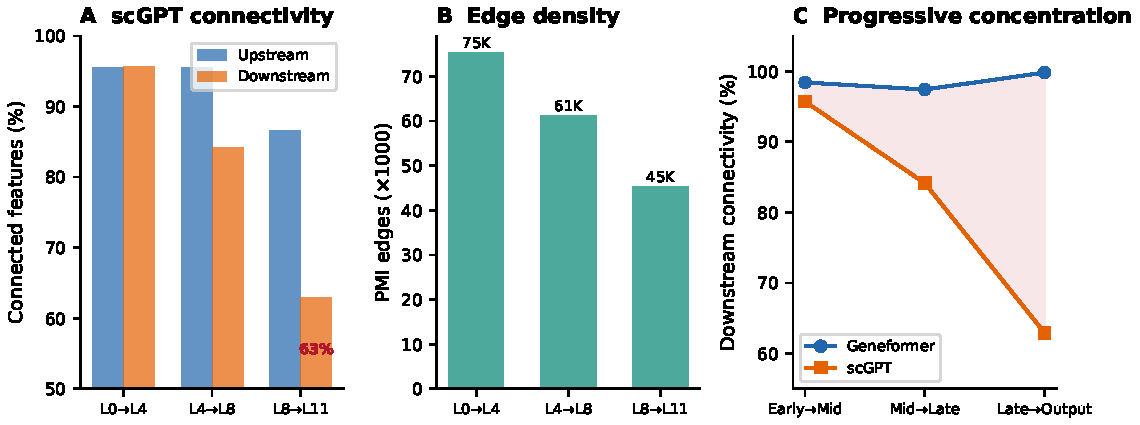
\includegraphics[width=\textwidth]{figures/gb_figS3_scgpt_highways.pdf}}
{\fbox{\parbox[c][3cm][c]{0.9\textwidth}{\centering FIGURE PENDING: \texttt{\detokenize{gb_figS3_scgpt_highways.pdf}}}}}
\caption{\textbf{scGPT cross-layer connectivity.} Upstream connectivity stays high while downstream connectivity falls with depth, a pattern Geneformer does not show.}
\label{fig:scgpt_highways}
\end{figure}

\begin{figure}[htbp]\centering
\IfFileExists{figures/gb_figS4_umap_overview.pdf}{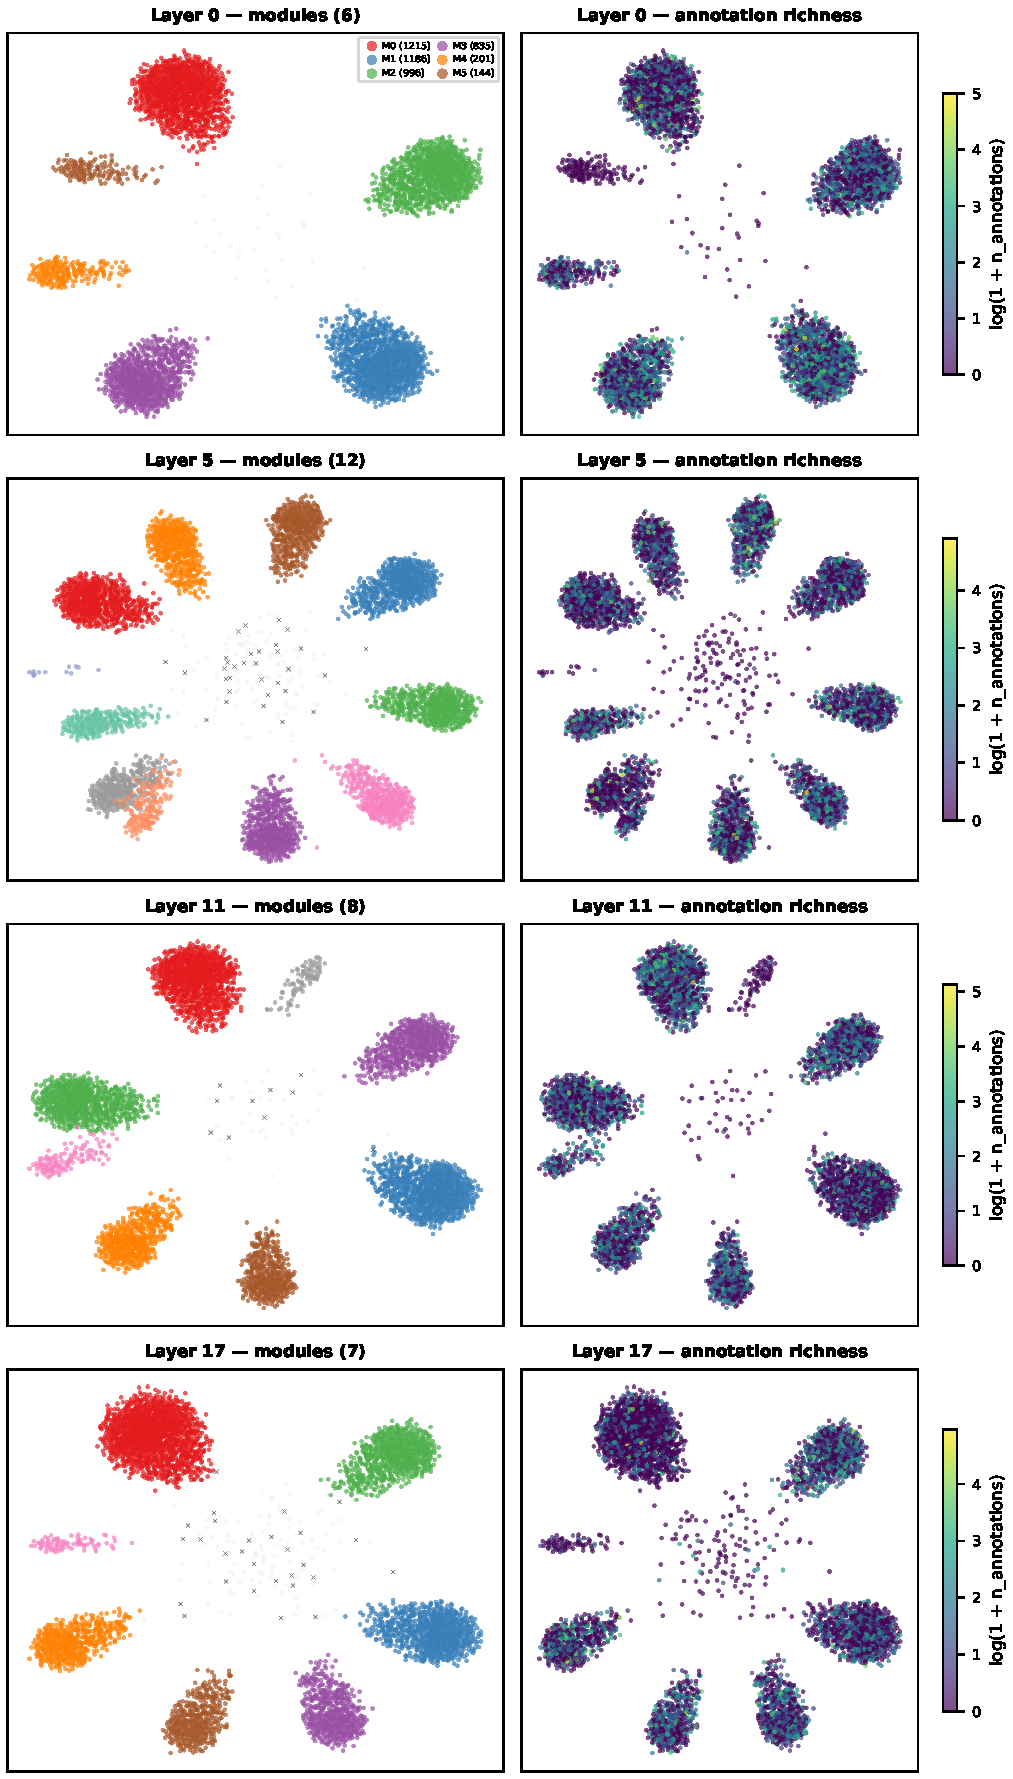
\includegraphics[width=\textwidth]{figures/gb_figS4_umap_overview.pdf}}
{\fbox{\parbox[c][3cm][c]{0.9\textwidth}{\centering FIGURE PENDING: \texttt{\detokenize{gb_figS4_umap_overview.pdf}}}}}
\caption{\textbf{Force-directed layout of the co-activation graph.} Each module forms a spatially coherent community. This is a layout of the co-activation graph, not a UMAP or t-SNE projection of the decoder directions.}
\label{fig:umap_overview}
\end{figure}

\begin{figure}[htbp]\centering
\IfFileExists{figures/gb_figS5_l11_detail.pdf}{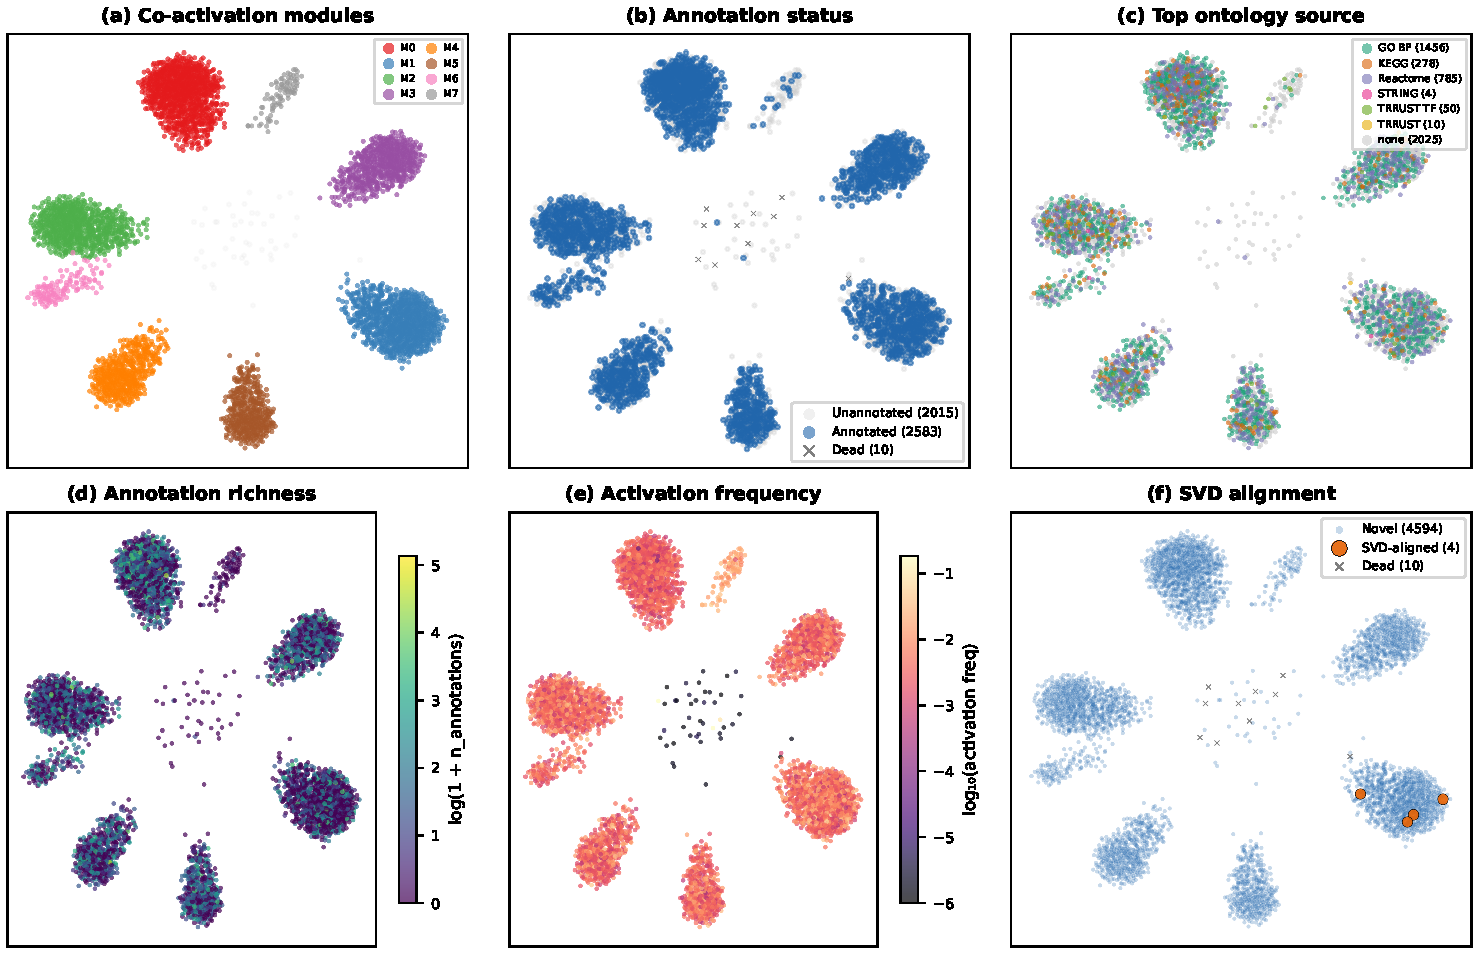
\includegraphics[width=\textwidth]{figures/gb_figS5_l11_detail.pdf}}
{\fbox{\parbox[c][3cm][c]{0.9\textwidth}{\centering FIGURE PENDING: \texttt{\detokenize{gb_figS5_l11_detail.pdf}}}}}
\caption{\textbf{Layer-11 co-activation graph in detail.} Annotated features distribute across all communities while sparsely annotated features concentrate centrally.}
\label{fig:l11_detail}
\end{figure}

\begin{figure}[htbp]\centering
\IfFileExists{figures/gb_figS6_annotation_projections.pdf}{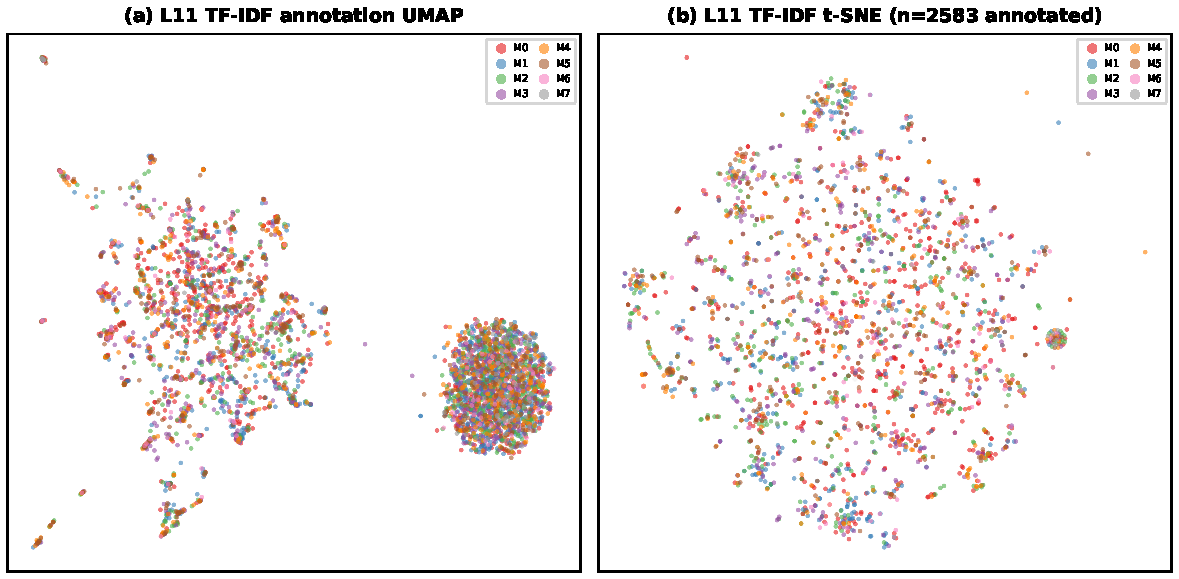
\includegraphics[width=\textwidth]{figures/gb_figS6_annotation_projections.pdf}}
{\fbox{\parbox[c][3cm][c]{0.9\textwidth}{\centering FIGURE PENDING: \texttt{\detokenize{gb_figS6_annotation_projections.pdf}}}}}
\caption{\textbf{Annotation-based projections.} TF-IDF weighted ontology vectors projected with UMAP and t-SNE, an independent check that module structure reflects biological similarity.}
\label{fig:annotation_projections}
\end{figure}

\end{document}

